% 2010 年广东卷文科第 14 题：直角梯形 ABCD。
% 来源 PDF：普通高考/2010/2010广东文.pdf，SHA-256 dd04b2053a22c854a9abe1ee03241fc04d5a25c91cda1d7997183bdfaa4a8c6f。
% 原页：第 1 页（A3 三栏）第 3 栏中部，书页码 595。
% 重绘依据：A(0,0)、B(4,0)、C(4,3.46)、D(2,3.46)；E 为 AB 中点，F 为 AD 中点。
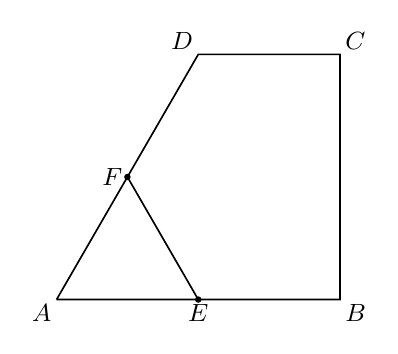
\begin{tikzpicture}[semithick, scale=0.9, every node/.style={inner sep=1.6pt, font=\small}]
  \coordinate (A) at (0,0);
  \coordinate (B) at (4,0);
  \coordinate (C) at (4,3.46);
  \coordinate (D) at (2,3.46);
  \coordinate (E) at (2,0);
  \coordinate (F) at (1,1.73);

  \draw (A) -- (B) -- (C) -- (D) -- (A);
  \draw (E) -- (F);
  \fill (E) circle (1.3pt);
  \fill (F) circle (1.3pt);
  \node[below left] at (A) {$A$};
  \node[below right] at (B) {$B$};
  \node[above right] at (C) {$C$};
  \node[above left] at (D) {$D$};
  \node[below] at (E) {$E$};
  \node[left] at (F) {$F$};
\end{tikzpicture}
